\documentclass[12pt]{article}
\usepackage{graphicx}
\usepackage[none]{hyphenat}
\usepackage[document]{ragged2e}
\usepackage[margin=1.0in]{geometry}

\usepackage{hyperref}
\hypersetup{
    colorlinks=true,
    linkcolor=blue,
    filecolor=magenta,      
    urlcolor=cyan,
    pdftitle={Quarter 1 Writeup},
    pdfpagemode=FullScreen,
}

\urlstyle{same}
\graphicspath {{./images/}}

\title{Predicting the Success of Baseball Pitchers \\ 
        \large Yilmaz Machine Learning 1 - 2022-2023}

\author{Wilson Chen and Bradley Cao}
\date{}
\begin{document}
\maketitle
\newpage{}
\section{Introduction}
\subsection{Overview}
For our project, we decided to look at a dataset on baseball pitchers. This dataset with 547 instances and 31 attributes contained information on different statistics recorded for pitchers. We wanted to see if we could use these statistics to predict whether or not a pitcher had a winning record. 

\subsection{Data Set}
We got our original dataset from REPLACE. It contained 31 attributes: 
\begin{itemize}
    \item $\textbf{last\_name}$
    \item $\textbf{first\_name}$
    \item $\textbf{player\_id}$
    \item $\textbf{year}$
    \item $\textbf{p\_game}$
    \item $\textbf{p\_total\_hits}$
    \item $\textbf{p\_home\_run}$
    \item $\textbf{p\_strikeout}$
    \item $\textbf{p\_walk}$
    \item $\textbf{p\_k\_percent}$
    \item $\textbf{p\_bb\_percent}$
    \item $\textbf{batting\_avg}$
    \item $\textbf{slg\_percent}$
    \item $\textbf{on\_base\_percent}$
    \item $\textbf{on\_base\_plus\_slg}$
    \item $\textbf{p\_earned\_run}$
    \item $\textbf{p\_win}$
    \item $\textbf{p\_loss}$
    \item $\textbf{p\_era}$
    \item $\textbf{p\_rbi}$
    \item $\textbf{p\_called\_strike}$
    \item $\textbf{p\_unearned\_run}$
    \item $\textbf{exit\_velocity\_avg}$
    \item $\textbf{launch\_angle\_avg}$
    \item $\textbf{sweet\_spot\_percent}$
    \item $\textbf{barrel\_batted\_rate}$
    \item $\textbf{hard\_hit\_percent}$
    \item $\textbf{meatball\_percent}$
    \item $\textbf{pitch\_hand}$
    \item $\textbf{n\_fastball\_formatted}$
    \item $\textbf{fastball\_avg\_speed}$
    \item $\textbf{n\_offspeed\_formatted}$
\end{itemize}
These attributes were collected by MLB or MLBStatCast, a partner company that specializes in collecting data from MLB games.  

\section{Preprocessing}
\subsection{Missing and Redundant Values}
We first started by removing redundant values, such as OPS. The OPS attribute is just the sum of the On Base Percentage ($\textbf{OBP}$) and Slugging ($\textbf{SLG}$), so we can safely remove it without losing any information. Furthermore, there were missing values for the attributes Offspeed\% and Offspeed Average MPH. We decided to remove these attributes altogether, as these values are missing because not all pitchers have an offspeed pitch; filling this data with an average would not be representative, and removing these attributes helps with dimensionality reduction. We also removed all attributes that did not relate to pitcher's performance ($\textbf{name}$, $\textbf{year}$, $\textbf{player}$ $\textbf{ID}$, etc.). 
\newpage{}
\subsection{Dimensionality Reduction}
We used WEKA's $\textbf{WrapperSubsetEval}$ technique with search method $\textbf{BestFit}$ to perform further dimensionality reduction. As shown in the screenshot below, the attibutes that were kept were $\textbf{p\_home\_run}$ (number of home runs given up), $\textbf{p\_strikeout}$ (number of strikeouts), $\textbf{p\_walk}$ (number of walks), $\textbf{batting\_avg}$ (batting average of opposing batters), $\textbf{slg\_percent}$ (slugging percent of opposing batters), and $\textbf{p\_era}$ (earned run average). 

\begin{figure}[h!]
    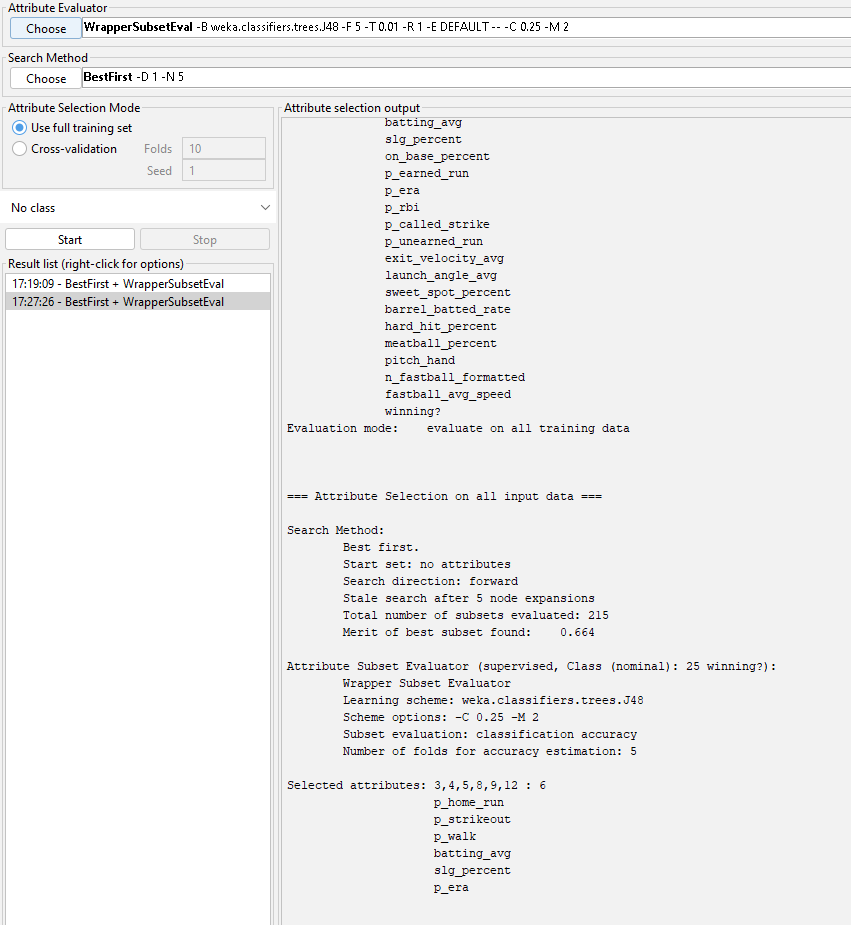
\includegraphics[scale=0.55]{DimRed.png}
    \caption{WEKA screenshot showing Dimensionality Reduction results}
    \label{fig:DimRed}
\end{figure}

\section{Splitting into Testing and Training}
After reducing dimensionality to these 7 attributes, we used WEKA to split our data into training and testing sets. We used WEKA's supervised method $\textbf{Resample}$, with sample size percent of 33\% and $\textbf{noReplacement}$ set to $\textbf{True}$. We ran it twice, once with $\textbf{invertSelection}$ set to $\textbf{False}$ to obtain our testing set. 
The second time, we ran it with $\textbf{invertSelection}$ set to $\textbf{True}$ to obtain our training set. 

\newpage
\begin{figure}[h!]
    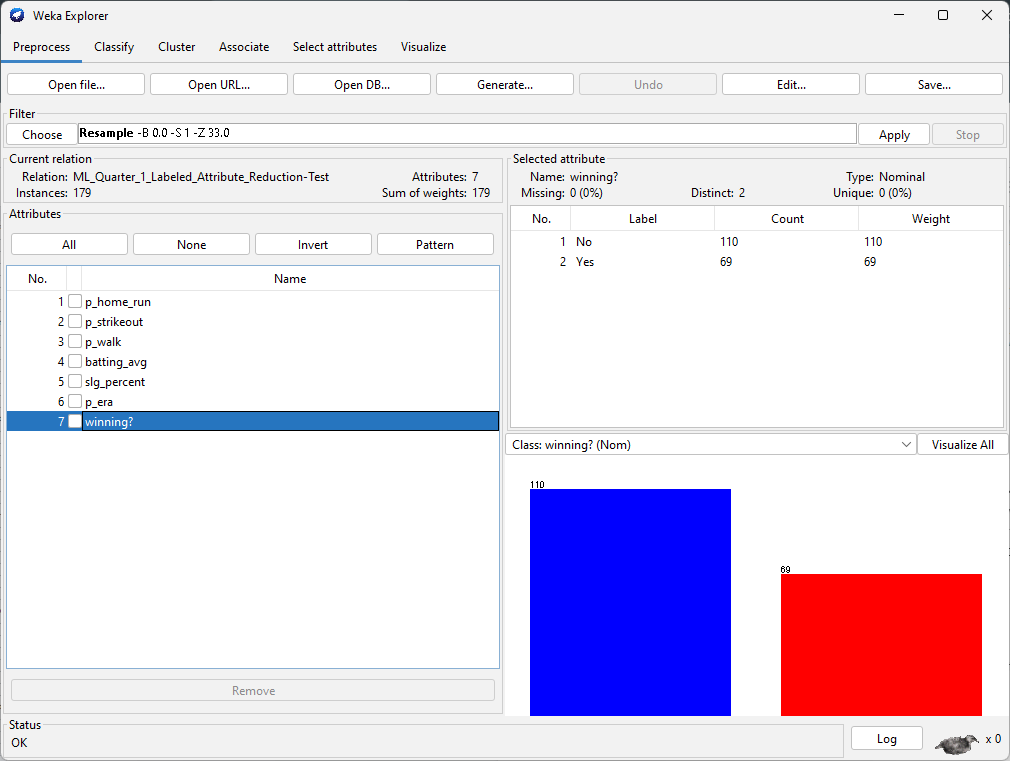
\includegraphics[scale=0.6]{TestSet.png}
    \caption{WEKA Screenshot showing the Testing Set}
    \label{fig:TestSet}
\end{figure}
\newpage
\begin{figure}[h!]
    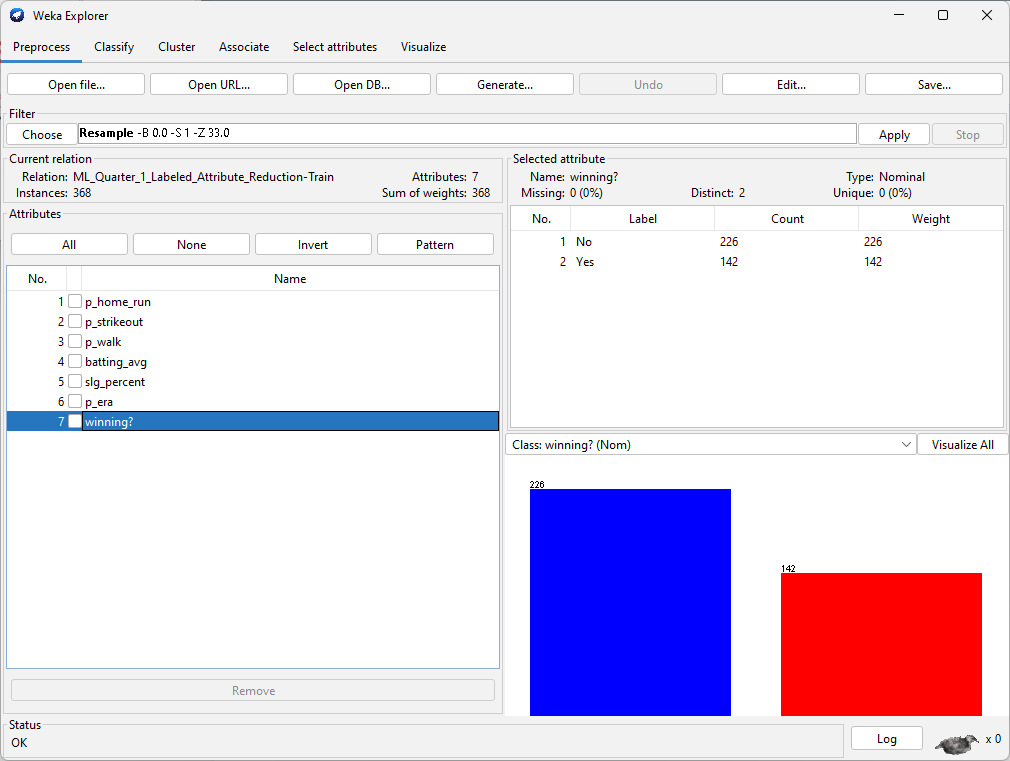
\includegraphics[scale=0.6]{TrainSet.png}
    \caption{WEKA Screenshot showing the Training Set}
    \label{fig:TrainSet}
\end{figure}

The class distribution of the testing and training sets can be seen in Figures 2 and 3. As seen by the class distributions, the WEKA $\textbf{Resample}$ method has maintained the non-uniform class distribution in the training and testing sets. This means that the 

\section{Classification}

\section{Discussion}

\section{Conclusion}

\section{Sources}
We got our data from \url{https://www.mlb.com} and used WEKA to preprocess and do classification work. 

\end{document}
